\documentclass{standalone}
\usepackage{tikz}
\usetikzlibrary{patterns, positioning}
\usepackage[sfdefault]{ClearSans} %% option 'sfdefault' activates Clear Sans as the default text font
\usepackage[T1]{fontenc}

\begin{document}
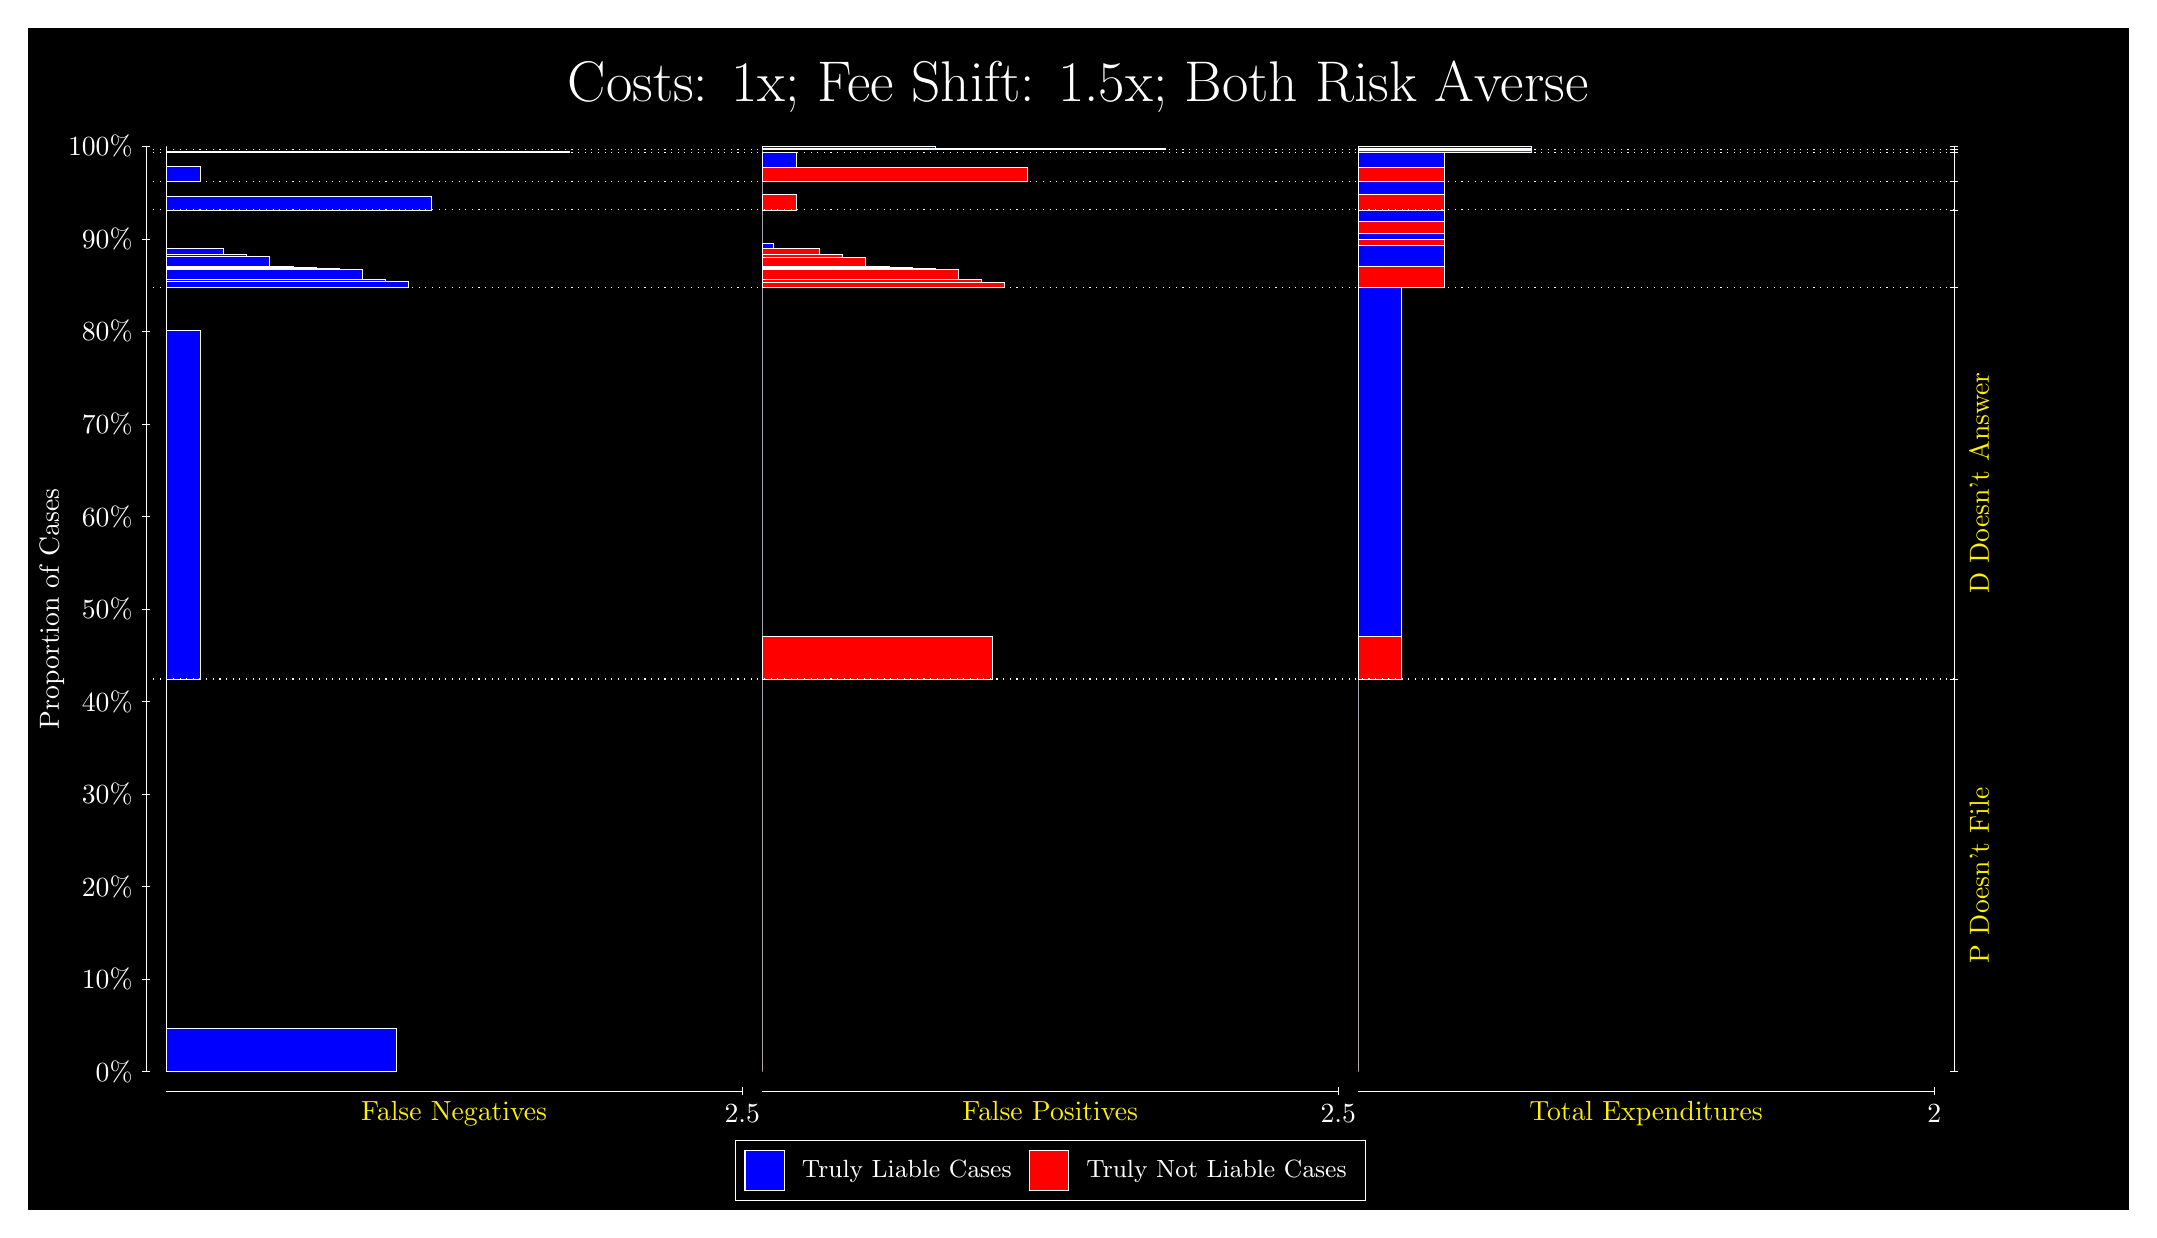
\begin{tikzpicture}
\draw[fill=black] (0,0) rectangle (26.667,15);
\draw[text=white] (0,13.5) rectangle (26.667,15) node[midway] {\huge Costs: 1x; Fee Shift: 1.5x; Both Risk Averse};
\draw[white, very thin] (1.5,1.75) -- (1.5,13.5);
\node[rotate=90, text=white, anchor=center] at (0.3, 7.625) {Proportion of Cases};
\draw[white, very thin] (1.45,1.75) -- (1.55,1.75);
\node[text=white, anchor=east] at (1.45, 1.75) {0\%};
\draw[white, very thin] (1.45,2.925) -- (1.55,2.925);
\node[text=white, anchor=east] at (1.45, 2.925) {10\%};
\draw[white, very thin] (1.45,4.1) -- (1.55,4.1);
\node[text=white, anchor=east] at (1.45, 4.1) {20\%};
\draw[white, very thin] (1.45,5.275) -- (1.55,5.275);
\node[text=white, anchor=east] at (1.45, 5.275) {30\%};
\draw[white, very thin] (1.45,6.45) -- (1.55,6.45);
\node[text=white, anchor=east] at (1.45, 6.45) {40\%};
\draw[white, very thin] (1.45,7.625) -- (1.55,7.625);
\node[text=white, anchor=east] at (1.45, 7.625) {50\%};
\draw[white, very thin] (1.45,8.8) -- (1.55,8.8);
\node[text=white, anchor=east] at (1.45, 8.8) {60\%};
\draw[white, very thin] (1.45,9.975) -- (1.55,9.975);
\node[text=white, anchor=east] at (1.45, 9.975) {70\%};
\draw[white, very thin] (1.45,11.15) -- (1.55,11.15);
\node[text=white, anchor=east] at (1.45, 11.15) {80\%};
\draw[white, very thin] (1.45,12.325) -- (1.55,12.325);
\node[text=white, anchor=east] at (1.45, 12.325) {90\%};
\draw[white, very thin] (1.45,13.5) -- (1.55,13.5);
\node[text=white, anchor=east] at (1.45, 13.5) {100\%};

\draw[white, very thin] (24.457,1.75) -- (24.457,13.5);
\draw[white, very thin] (24.407,1.75) -- (24.507,1.75);
\node[anchor=west] at (24.407, 1.75) {};
\draw[white, very thin] (24.407,6.7356) -- (24.507,6.7356);
\node[anchor=west] at (24.407, 6.7356) {};
\draw[white, very thin] (24.407,11.711) -- (24.507,11.711);
\node[anchor=west] at (24.407, 11.711) {};
\draw[white, very thin] (24.407,12.693) -- (24.507,12.693);
\node[anchor=west] at (24.407, 12.693) {};
\draw[white, very thin] (24.407,13.057) -- (24.507,13.057);
\node[anchor=west] at (24.407, 13.057) {};
\draw[white, very thin] (24.407,13.42) -- (24.507,13.42);
\node[anchor=west] at (24.407, 13.42) {};
\draw[white, very thin] (24.407,13.46) -- (24.507,13.46);
\node[anchor=west] at (24.407, 13.46) {};
\draw[white, very thin] (24.407,13.5) -- (24.507,13.5);
\node[anchor=west] at (24.407, 13.5) {};

\draw[white, very thin, fill=blue] (1.75,1.75) rectangle (4.6775,2.2987);
\draw[white, very thin, fill=red] (1.75,2.2987) rectangle (1.75,6.7356);
\draw[white, very thin, fill=blue] (1.75,6.7356) rectangle (2.1891,11.167);
\draw[white, very thin, fill=red] (1.75,11.167) rectangle (1.75,11.711);
\draw[white, very thin, fill=blue] (1.75,11.711) rectangle (4.8239,11.782);
\draw[white, very thin, fill=blue] (1.75,11.782) rectangle (4.5312,11.815);
\draw[white, very thin, fill=blue] (1.75,11.815) rectangle (4.2384,11.933);
\draw[white, very thin, fill=blue] (1.75,11.933) rectangle (3.9457,11.945);
\draw[white, very thin, fill=blue] (1.75,11.945) rectangle (3.6529,11.964);
\draw[white, very thin, fill=blue] (1.75,11.964) rectangle (3.3602,11.976);
\draw[white, very thin, fill=blue] (1.75,11.976) rectangle (3.0674,12.101);
\draw[white, very thin, fill=blue] (1.75,12.101) rectangle (2.7746,12.134);
\draw[white, very thin, fill=blue] (1.75,12.134) rectangle (2.4819,12.202);
\draw[white, very thin, fill=red] (1.75,12.202) rectangle (1.75,12.693);
\draw[white, very thin, fill=blue] (1.75,12.693) rectangle (5.1167,12.865);
\draw[white, very thin, fill=red] (1.75,12.865) rectangle (1.75,13.057);
\draw[white, very thin, fill=blue] (1.75,13.057) rectangle (2.1891,13.249);
\draw[white, very thin, fill=red] (1.75,13.249) rectangle (1.75,13.42);
\draw[white, very thin, fill=blue] (1.75,13.42) rectangle (6.8732,13.436);
\draw[white, very thin, fill=red] (1.75,13.436) rectangle (1.75,13.46);
\draw[white, very thin, fill=red] (1.75,13.46) rectangle (1.75,13.476);
\draw[white, very thin, fill=blue] (1.75,13.476) rectangle (1.75,13.5);
\draw[white, very thin, fill=red] (9.3189,1.75) rectangle (9.3189,6.1869);
\draw[white, very thin, fill=blue] (9.3189,6.1869) rectangle (9.3189,6.7356);
\draw[white, very thin, fill=red] (9.3189,6.7356) rectangle (12.246,7.2792);
\draw[white, very thin, fill=blue] (9.3189,7.2792) rectangle (9.3189,11.711);
\draw[white, very thin, fill=red] (9.3189,11.711) rectangle (12.393,11.775);
\draw[white, very thin, fill=red] (9.3189,11.775) rectangle (12.1,11.808);
\draw[white, very thin, fill=red] (9.3189,11.808) rectangle (11.807,11.933);
\draw[white, very thin, fill=red] (9.3189,11.933) rectangle (11.515,11.945);
\draw[white, very thin, fill=red] (9.3189,11.945) rectangle (11.222,11.964);
\draw[white, very thin, fill=red] (9.3189,11.964) rectangle (10.929,11.976);
\draw[white, very thin, fill=red] (9.3189,11.976) rectangle (10.636,12.094);
\draw[white, very thin, fill=red] (9.3189,12.094) rectangle (10.344,12.127);
\draw[white, very thin, fill=red] (9.3189,12.127) rectangle (10.051,12.202);
\draw[white, very thin, fill=blue] (9.3189,12.202) rectangle (9.4652,12.27);
\draw[white, very thin, fill=blue] (9.3189,12.27) rectangle (9.3189,12.693);
\draw[white, very thin, fill=red] (9.3189,12.693) rectangle (9.758,12.885);
\draw[white, very thin, fill=blue] (9.3189,12.885) rectangle (9.3189,13.057);
\draw[white, very thin, fill=red] (9.3189,13.057) rectangle (12.686,13.229);
\draw[white, very thin, fill=blue] (9.3189,13.229) rectangle (9.758,13.42);
\draw[white, very thin, fill=red] (9.3189,13.42) rectangle (9.3189,13.444);
\draw[white, very thin, fill=blue] (9.3189,13.444) rectangle (9.3189,13.46);
\draw[white, very thin, fill=red] (9.3189,13.46) rectangle (14.442,13.476);
\draw[white, very thin, fill=blue] (9.3189,13.476) rectangle (11.515,13.5);
\draw[white, very thin, fill=red] (16.888,1.75) rectangle (16.888,6.1869);
\draw[white, very thin, fill=blue] (16.888,6.1869) rectangle (16.888,6.7356);
\draw[white, very thin, fill=red] (16.888,6.7356) rectangle (17.437,7.2792);
\draw[white, very thin, fill=blue] (16.888,7.2792) rectangle (17.437,11.711);
\draw[white, very thin, fill=red] (16.888,11.711) rectangle (17.986,11.976);
\draw[white, very thin, fill=blue] (16.888,11.976) rectangle (17.986,12.246);
\draw[white, very thin, fill=red] (16.888,12.246) rectangle (17.986,12.32);
\draw[white, very thin, fill=blue] (16.888,12.32) rectangle (17.986,12.391);
\draw[white, very thin, fill=red] (16.888,12.391) rectangle (17.986,12.542);
\draw[white, very thin, fill=blue] (16.888,12.542) rectangle (17.986,12.693);
\draw[white, very thin, fill=red] (16.888,12.693) rectangle (17.986,12.885);
\draw[white, very thin, fill=blue] (16.888,12.885) rectangle (17.986,13.057);
\draw[white, very thin, fill=red] (16.888,13.057) rectangle (17.986,13.229);
\draw[white, very thin, fill=blue] (16.888,13.229) rectangle (17.986,13.42);
\draw[white, very thin, fill=red] (16.888,13.42) rectangle (19.083,13.444);
\draw[white, very thin, fill=blue] (16.888,13.444) rectangle (19.083,13.46);
\draw[white, very thin, fill=red] (16.888,13.46) rectangle (19.083,13.476);
\draw[white, very thin, fill=blue] (16.888,13.476) rectangle (19.083,13.5);
\draw[white, dotted] (1.5,6.7356) -- (24.457,6.7356);
\draw[white, dotted] (1.5,11.711) -- (24.457,11.711);
\draw[white, dotted] (1.5,12.693) -- (24.457,12.693);
\draw[white, dotted] (1.5,13.057) -- (24.457,13.057);
\draw[white, dotted] (1.5,13.42) -- (24.457,13.42);
\draw[white, dotted] (1.5,13.46) -- (24.457,13.46);
\draw[white, very thin] (1.75,1.5) -- (9.0689,1.5);
\node[text=yellow, anchor=north] at (5.4094, 1.5) {False Negatives};
\draw[white, very thin] (9.0689,1.45) -- (9.0689,1.55);
\node[text=white, anchor=north] at (9.0689, 1.45) {2.5};

\draw[white, very thin] (9.3189,1.5) -- (16.638,1.5);
\node[text=yellow, anchor=north] at (12.978, 1.5) {False Positives};
\draw[white, very thin] (16.638,1.45) -- (16.638,1.55);
\node[text=white, anchor=north] at (16.638, 1.45) {2.5};

\draw[white, very thin] (16.888,1.5) -- (24.207,1.5);
\node[text=yellow, anchor=north] at (20.547, 1.5) {Total Expenditures};
\draw[white, very thin] (24.207,1.45) -- (24.207,1.55);
\node[text=white, anchor=north] at (24.207, 1.45) {2};

\node[text=yellow, centered, rotate=90] at (24.777, 4.2428) {P Doesn't File};
\node[text=yellow, centered, rotate=90] at (24.777, 9.2233) {D Doesn't Answer};






\draw (12.978300999999998,1.5) node[draw=none] (baseCoordinate) {};
\begin{scope}[align=center]
        \matrix[scale=0.5, draw=white, below=0.5cm of baseCoordinate, nodes={draw}, column sep=0.1cm]{
            \node[rectangle, draw, minimum width=0.5cm, minimum height=0.5cm, fill=blue] {}; &
            \node[draw=none, font=\small, text=white] (B) {Truly Liable Cases}; &
            \node[rectangle, draw, minimum width=0.5cm, minimum height=0.5cm, fill=red] {}; &
            \node[draw=none, font=\small, text=white] (B) {Truly Not Liable Cases}; \\
            };
\end{scope}

\end{tikzpicture}
\end{document}